\section{Einleitung}
Mit dem Versuch "Vermessung von szintillierenden Fasern für das LHCb-Experiment" sollen die Messeigenschaften von szintillierenden Fasern untersucht und mit Simulationsdaten verglichen werden. Im Anschluss wird die Simulation anhand der Messdaten an die Realität angepasst.

\section{Theorie}
Szintillierende Fasern finden ihren Einsatz beispielsweise im LHCb-Experiment, wo sie im Zuge des Upgrades in einem der Spurdetektoren platziert werden.
Dort sind sie in Fasermatten angeordnet, welche aus einer hexagonalen Anordnung der einzelnen Fasern bestehen. Die einzelnen Matten werden in 4 Lagen mit je 2 Reihen von 40 nebeneinander liegenden Matten angeordnet. Hierbei sind die beiden inneren Lagen um $\SI{5}{°}$ gegenüber den äußeren Lagen geneigt. Dadurch wird die überlappende Fläche minimiert, womit eine hohe Ortsauflösung der Fasern von unter $\SI{100}{\micro m}$ erreicht wird. 

Eine hohe Ortsauflösung ist elementar für eine genaue Spurrekonstruktion. Aus Krümmungsradien der Spuren in einem Magnetfeld kann der Impuls der detektierten Teilchen bestimmt werden. Dies ist eine wichtige Messvariable, welche in Kombination mit Informationen aus anderen Detektorbestandteilen zur Identifikation der Teilchen dient. 

\subsection{Szintillationsmechanismus}
Der Kern einer Faser besteht aus dem organischen Szintillatormaterial Polystyrol und hat eine Dicke von $\SI{220}{\micro m}$. Gelangt ein ionisierendes Teilchen in den Faserkern, löst es Valenzbandelektronen aus ihren Atombindungen und hebt sie auf ein erhöhtes Energieniveau.
\begin{wrapfigure}[16]{r}{0.5\textwidth}
  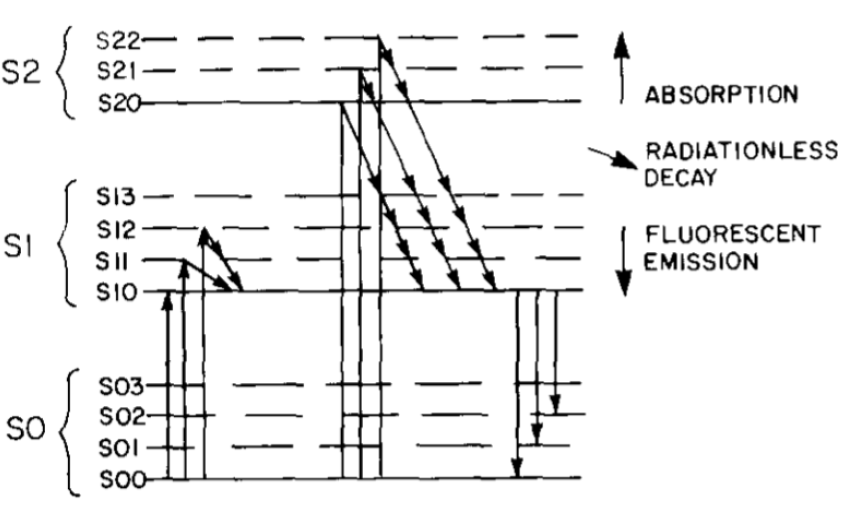
\includegraphics[width=0.48\textwidth]{plots/Energieniveaus.png}
  \caption{Energieniveaus des szintillierenden Materials Polystyrol. Lediglich der Übergang von S$_{10}$ in S$_{00}$ erfolgt unter Emission vom elektromagnetischer Strahlung \cite{anleitung}.}
  \label{fig:Niveaus}
\end{wrapfigure}
\FloatBarrier
Die Elektronen relaxieren anschließend in den Grundzustand zurück, wobei die meisten Übergänge strahlungsfrei erfolgen. Lediglich bei einem Übergang vom ersten angeregten Zustand S$_{10}$ in den Grundzustand S$_{00}$ werden Photonen im UV-Bereich emittiert. Dieser ist relativ unwahrscheinlich im Verhältnis zu den strahlungsfreien Übergängen, sodass lediglich bei 3$\;\%$ der ionisierenden Teilchen ein Photon erzeugt wird.

Um die Quantenausbeute zu steigern wird dem Polystyrol der Farbstoff p-Terphenyl hinzugefügt. Die Polystyrolmoleküle übertragen ihre Energie über Dipol-Dipol-Wechselwirkungen an die Farbstoffmoleküle, welche anschließend unter Emission von Photonen relaxieren. 

\subsection{Photonenleitung}
\label{theorie}
Die Photonen werden dann entlang der Faser zu ihren äußeren Enden geleitet, wo sie mit Hilfe von Photomultipliern detektiert werden. Um zu verhindern, dass die Photonen den Kern zuvor verlassen, befinden sich um den Kern zwei Mantelschichten. Diese besitzen nach außen abnehmende Brechnungsindices, sodass die Photonen an den Grenzflächen total reflektiert werden. Der Winkel $\theta$ beschreibt dabei den Winkel des Photons zur $x$-Achse, welche, wie Abbildung \ref{fig:Geometrie} zu entnehmen, entlang der Längsachse der Faser verläuft.
\begin{figure}
    \centering
    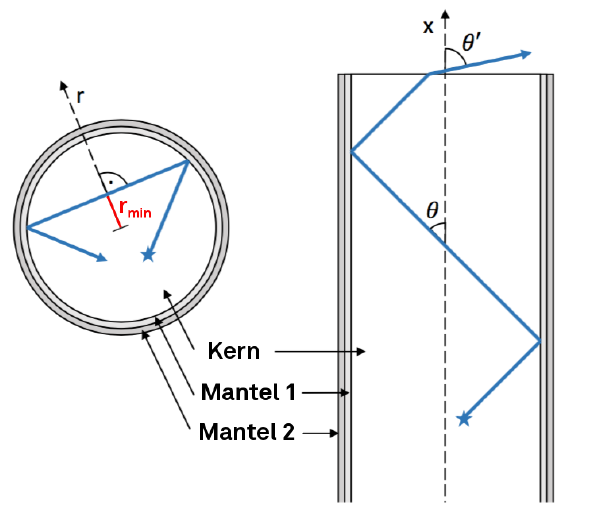
\includegraphics[width=0.5\textwidth]{plots/Geometrie.png}
    \caption{Links: Querschnitt durch die Faser mit beispielhaften Weg des Photons durch die Faser (blau). Rechts: Längsschnitt durch die Faser mit beispielhaften Weg des Photons durch die Faser (blau) \cite{anleitung}.}
    \label{fig:Geometrie}
  \end{figure} 
Für die Wegstrecke des Photons im Faserkern kann über Winkelrelationen der Zusammenhang 
\begin{align}
    L = \frac{x}{\cos(\theta)}
    \label{eq:1.1}
\end{align}
hergeleitet werden, wobei $x$ den Abstand zum Faserende beschreibt. Die Anzahl an Reflektionen auf dieser Strecke kann über 
\begin{align}
    N = \frac{x \tan(\theta)}{2 \sqrt{r_\mathrm{Kern}^2 - r_\mathrm{min}^2}}
    \label{eq:1.2}
\end{align}
ermittelt werden. $r_\mathrm{Kern}^2$ ist dabei durch den Radius des Kernes und $r_\mathrm{min}^2$, wie Abbildung \ref{fig:Geometrie} zu entnehmen, durch den kleinsten Abstand des Photons zur Mittelachse gegeben. Der Reflektionswinkel, unter welchem das Photon Totalreflektion begeht, wird durch den Zusammenhang 
\begin{align}
    \theta_\mathrm{refl} = \arcsin\left( \sqrt{1 - \frac{r_\mathrm{min}^2}{r_\mathrm{Kern}^2}} \sin(\theta)\right)
    \label{eq:2}
\end{align}
beschrieben. 
%----------Maximales Theta für Totalreflektion-------------?

Da die Abschwächlänge der emittierten Photonen im Polystyrol-Farbstoff-Gemisch zu gering ist, um das Faserende zu erreichen, wird der Faser ein Wellenlängenschieber in Form des Materials Tetraphenyl butadiene zugefügt. Dieses absorbiert die Photonen und emittiert sie erneut mit einer höheren Wellenlänge.

Trotz dieser Maßnahme erreichen nicht alle Photonen die Ausleseelektronik am Faserende. Neben Reflektionen am Faserende und an den Grenzflächen zum Mantel können die Photonen durch Streuung und Absorption im Kernmaterial verloren gehen. Die Abschwächung der Photonenintensität erfolt logarithmisch mit dem Absorbtionskoeffizienten der Wechselwirkungen, welche in Abbildung \ref{fig:ww} für die einzelnen Prozesse in Abhängigkeit von der Wellenlänge aufgetragen sind.\\
\begin{wrapfigure}[15]{r}{0.5\textwidth}
    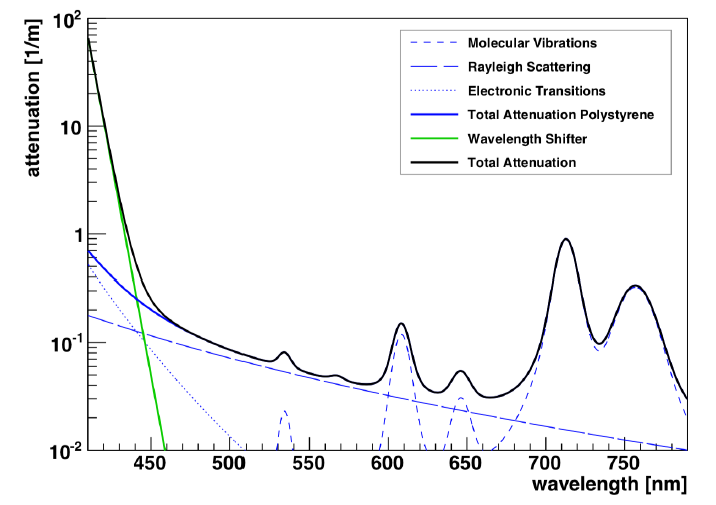
\includegraphics[width=0.48\textwidth]{plots/Absorption.png}
    \caption{Absorptionskoeffizienten in Abhängigkeit von der Wellenlänge für die Prozesse, welche zu einer Abschwächung der Photonenintensität im Faserkern führen \cite{anleitung}.}
    \label{fig:ww}
  \end{wrapfigure}
  \FloatBarrier
Aufgrund der verschiedenen Winkelabhängigkeiten der Wechselwirkungen kann der Gesamtabsorptionskoeffizient in einen Kern- und einen Reflektionsanteil aufgeteilt werden. Somit lässt sich zusammengefasst der Absorptionskoeffizient als 
\begin{align}
    a_\mathrm{eff} = \frac{a_0}{\cos(\theta)} + \frac{\epsilon \tan(\theta)}{2 \sqrt{r_\mathrm{Kern}^2 - r_\mathrm{min}^2}}
    \label{eq:9}
\end{align}
darstellen. Hierbei beschreibt $\epsilon$ den Rreflexionskoeffizienten und $a_0$ ???.

\subsection{Ausleseelektronik}
Die Photonen werden am Faserende durch Avalanche-Photodioden. Diese bestehen aus $(57.7 \times 62.5)\;\si{\micro m}$ großen Pixeln, welche durch einzelne pn-Übergänge in Sperrrichtung realisiert werden. Trifft ein Photon auf die Sperrzone einer Diode, erzeugt es Elektron-Loch-Paare, welche zu den jeweiligen Polen hin beschleunigt werden. Hierbei erfahren sie eine so hohe Beschleunigung, dass sie weitere freie Ladungsträger erzeugen und eine Lawine an Elektron-Loch-Paaren entsteht. Diese rufen einen Ladungsimpuls an den Polen hervor, welche durch die Elektronik weiter verarbeitet werden kann.

Über die Anzahl und Position der gefeuerten Pixel kann die Stelle bestimmt werden, an welcher das Photon die Faser verlassen hat. Zur Messung der Wellenlänge oder einer Winkelabhänigikeit der Photonen werden Spektrometer eingesetzt. 